% Options for packages loaded elsewhere
\PassOptionsToPackage{unicode}{hyperref}
\PassOptionsToPackage{hyphens}{url}
%
\documentclass[
]{book}
\usepackage{amsmath,amssymb}
\usepackage{lmodern}
\usepackage{iftex}
\ifPDFTeX
  \usepackage[T1]{fontenc}
  \usepackage[utf8]{inputenc}
  \usepackage{textcomp} % provide euro and other symbols
\else % if luatex or xetex
  \usepackage{unicode-math}
  \defaultfontfeatures{Scale=MatchLowercase}
  \defaultfontfeatures[\rmfamily]{Ligatures=TeX,Scale=1}
\fi
% Use upquote if available, for straight quotes in verbatim environments
\IfFileExists{upquote.sty}{\usepackage{upquote}}{}
\IfFileExists{microtype.sty}{% use microtype if available
  \usepackage[]{microtype}
  \UseMicrotypeSet[protrusion]{basicmath} % disable protrusion for tt fonts
}{}
\makeatletter
\@ifundefined{KOMAClassName}{% if non-KOMA class
  \IfFileExists{parskip.sty}{%
    \usepackage{parskip}
  }{% else
    \setlength{\parindent}{0pt}
    \setlength{\parskip}{6pt plus 2pt minus 1pt}}
}{% if KOMA class
  \KOMAoptions{parskip=half}}
\makeatother
\usepackage{xcolor}
\usepackage{color}
\usepackage{fancyvrb}
\newcommand{\VerbBar}{|}
\newcommand{\VERB}{\Verb[commandchars=\\\{\}]}
\DefineVerbatimEnvironment{Highlighting}{Verbatim}{commandchars=\\\{\}}
% Add ',fontsize=\small' for more characters per line
\usepackage{framed}
\definecolor{shadecolor}{RGB}{248,248,248}
\newenvironment{Shaded}{\begin{snugshade}}{\end{snugshade}}
\newcommand{\AlertTok}[1]{\textcolor[rgb]{0.94,0.16,0.16}{#1}}
\newcommand{\AnnotationTok}[1]{\textcolor[rgb]{0.56,0.35,0.01}{\textbf{\textit{#1}}}}
\newcommand{\AttributeTok}[1]{\textcolor[rgb]{0.77,0.63,0.00}{#1}}
\newcommand{\BaseNTok}[1]{\textcolor[rgb]{0.00,0.00,0.81}{#1}}
\newcommand{\BuiltInTok}[1]{#1}
\newcommand{\CharTok}[1]{\textcolor[rgb]{0.31,0.60,0.02}{#1}}
\newcommand{\CommentTok}[1]{\textcolor[rgb]{0.56,0.35,0.01}{\textit{#1}}}
\newcommand{\CommentVarTok}[1]{\textcolor[rgb]{0.56,0.35,0.01}{\textbf{\textit{#1}}}}
\newcommand{\ConstantTok}[1]{\textcolor[rgb]{0.00,0.00,0.00}{#1}}
\newcommand{\ControlFlowTok}[1]{\textcolor[rgb]{0.13,0.29,0.53}{\textbf{#1}}}
\newcommand{\DataTypeTok}[1]{\textcolor[rgb]{0.13,0.29,0.53}{#1}}
\newcommand{\DecValTok}[1]{\textcolor[rgb]{0.00,0.00,0.81}{#1}}
\newcommand{\DocumentationTok}[1]{\textcolor[rgb]{0.56,0.35,0.01}{\textbf{\textit{#1}}}}
\newcommand{\ErrorTok}[1]{\textcolor[rgb]{0.64,0.00,0.00}{\textbf{#1}}}
\newcommand{\ExtensionTok}[1]{#1}
\newcommand{\FloatTok}[1]{\textcolor[rgb]{0.00,0.00,0.81}{#1}}
\newcommand{\FunctionTok}[1]{\textcolor[rgb]{0.00,0.00,0.00}{#1}}
\newcommand{\ImportTok}[1]{#1}
\newcommand{\InformationTok}[1]{\textcolor[rgb]{0.56,0.35,0.01}{\textbf{\textit{#1}}}}
\newcommand{\KeywordTok}[1]{\textcolor[rgb]{0.13,0.29,0.53}{\textbf{#1}}}
\newcommand{\NormalTok}[1]{#1}
\newcommand{\OperatorTok}[1]{\textcolor[rgb]{0.81,0.36,0.00}{\textbf{#1}}}
\newcommand{\OtherTok}[1]{\textcolor[rgb]{0.56,0.35,0.01}{#1}}
\newcommand{\PreprocessorTok}[1]{\textcolor[rgb]{0.56,0.35,0.01}{\textit{#1}}}
\newcommand{\RegionMarkerTok}[1]{#1}
\newcommand{\SpecialCharTok}[1]{\textcolor[rgb]{0.00,0.00,0.00}{#1}}
\newcommand{\SpecialStringTok}[1]{\textcolor[rgb]{0.31,0.60,0.02}{#1}}
\newcommand{\StringTok}[1]{\textcolor[rgb]{0.31,0.60,0.02}{#1}}
\newcommand{\VariableTok}[1]{\textcolor[rgb]{0.00,0.00,0.00}{#1}}
\newcommand{\VerbatimStringTok}[1]{\textcolor[rgb]{0.31,0.60,0.02}{#1}}
\newcommand{\WarningTok}[1]{\textcolor[rgb]{0.56,0.35,0.01}{\textbf{\textit{#1}}}}
\usepackage{longtable,booktabs,array}
\usepackage{calc} % for calculating minipage widths
% Correct order of tables after \paragraph or \subparagraph
\usepackage{etoolbox}
\makeatletter
\patchcmd\longtable{\par}{\if@noskipsec\mbox{}\fi\par}{}{}
\makeatother
% Allow footnotes in longtable head/foot
\IfFileExists{footnotehyper.sty}{\usepackage{footnotehyper}}{\usepackage{footnote}}
\makesavenoteenv{longtable}
\usepackage{graphicx}
\makeatletter
\def\maxwidth{\ifdim\Gin@nat@width>\linewidth\linewidth\else\Gin@nat@width\fi}
\def\maxheight{\ifdim\Gin@nat@height>\textheight\textheight\else\Gin@nat@height\fi}
\makeatother
% Scale images if necessary, so that they will not overflow the page
% margins by default, and it is still possible to overwrite the defaults
% using explicit options in \includegraphics[width, height, ...]{}
\setkeys{Gin}{width=\maxwidth,height=\maxheight,keepaspectratio}
% Set default figure placement to htbp
\makeatletter
\def\fps@figure{htbp}
\makeatother
\setlength{\emergencystretch}{3em} % prevent overfull lines
\providecommand{\tightlist}{%
  \setlength{\itemsep}{0pt}\setlength{\parskip}{0pt}}
\setcounter{secnumdepth}{5}
\usepackage{booktabs}
\ifLuaTeX
  \usepackage{selnolig}  % disable illegal ligatures
\fi
\usepackage[]{natbib}
\bibliographystyle{plainnat}
\IfFileExists{bookmark.sty}{\usepackage{bookmark}}{\usepackage{hyperref}}
\IfFileExists{xurl.sty}{\usepackage{xurl}}{} % add URL line breaks if available
\urlstyle{same} % disable monospaced font for URLs
\hypersetup{
  pdftitle={行動経済学の実証分析},
  pdfauthor={Tomohisa OKADA},
  hidelinks,
  pdfcreator={LaTeX via pandoc}}

\title{行動経済学の実証分析}
\author{Tomohisa OKADA}
\date{2023-04-26}

\begin{document}
\maketitle

{
\setcounter{tocdepth}{1}
\tableofcontents
}
\hypertarget{ready}{%
\chapter{Ready?}\label{ready}}

\hypertarget{rstudioux3068ux306f}{%
\section{R(Studio)とは?}\label{rstudioux3068ux306f}}

\begin{itemize}
\tightlist
\item
  Rは、オープンソースで利用可能な統計解析に特化したプログラミング言語
\item
  RStudioは、Rを使うための統合開発環境(なくてもRは使えるが、あるとめちゃ便利!)
\end{itemize}

\hypertarget{tips}{%
\section{Tips!}\label{tips}}

\begin{itemize}
\tightlist
\item
  Rに関するお役立ちサイトや書籍をまとめる
\end{itemize}

\begin{enumerate}
\def\labelenumi{\arabic{enumi}.}
\item
  \href{https://tomoecon.github.io/R_for_graduate_thesis/}{「卒業論文のためのR入門」 by 森知春先生}\\
  Rの使い方と心理統計学の基礎が一挙に学べる!
\item
  \href{https://www.jaysong.net/RBook/datahandling1.html}{「私たちのR」 by 宋財泫先生 \& 矢内勇生先生}\\
  辞書的に使える!Tidyverseを使ったモダンなRのプログラムが学べる!
\end{enumerate}

\hypertarget{rstudioux306eux30a4ux30f3ux30b9ux30c8ux30fcux30eb}{%
\section{R(Studio)のインストール}\label{rstudioux306eux30a4ux30f3ux30b9ux30c8ux30fcux30eb}}

\begin{itemize}
\tightlist
\item
  次のサイトにアクセス( \url{https://posit.co/download/rstudio-desktop/} )
\item
  「1:Install R」からRをインストール
\item
  「2:Install RStudio」からRStudioをインストール
\item
  うまくインストールできない場合は、\href{https://www.jaysong.net/RBook/installation.html}{「私たちのR」}に詳しい解説がある
\end{itemize}

\hypertarget{go}{%
\chapter{Go!!}\label{go}}

\begin{itemize}
\tightlist
\item
  とりあえずまずは使ってみよう!
\end{itemize}

\hypertarget{rstudioux3092ux958bux304f}{%
\section{RStudioを開く}\label{rstudioux3092ux958bux304f}}

\begin{itemize}
\tightlist
\item
  RStudioのアイコンから起動
\item
  次のような、4つの枠(ペーン)に分かれた画面が表示される
\end{itemize}

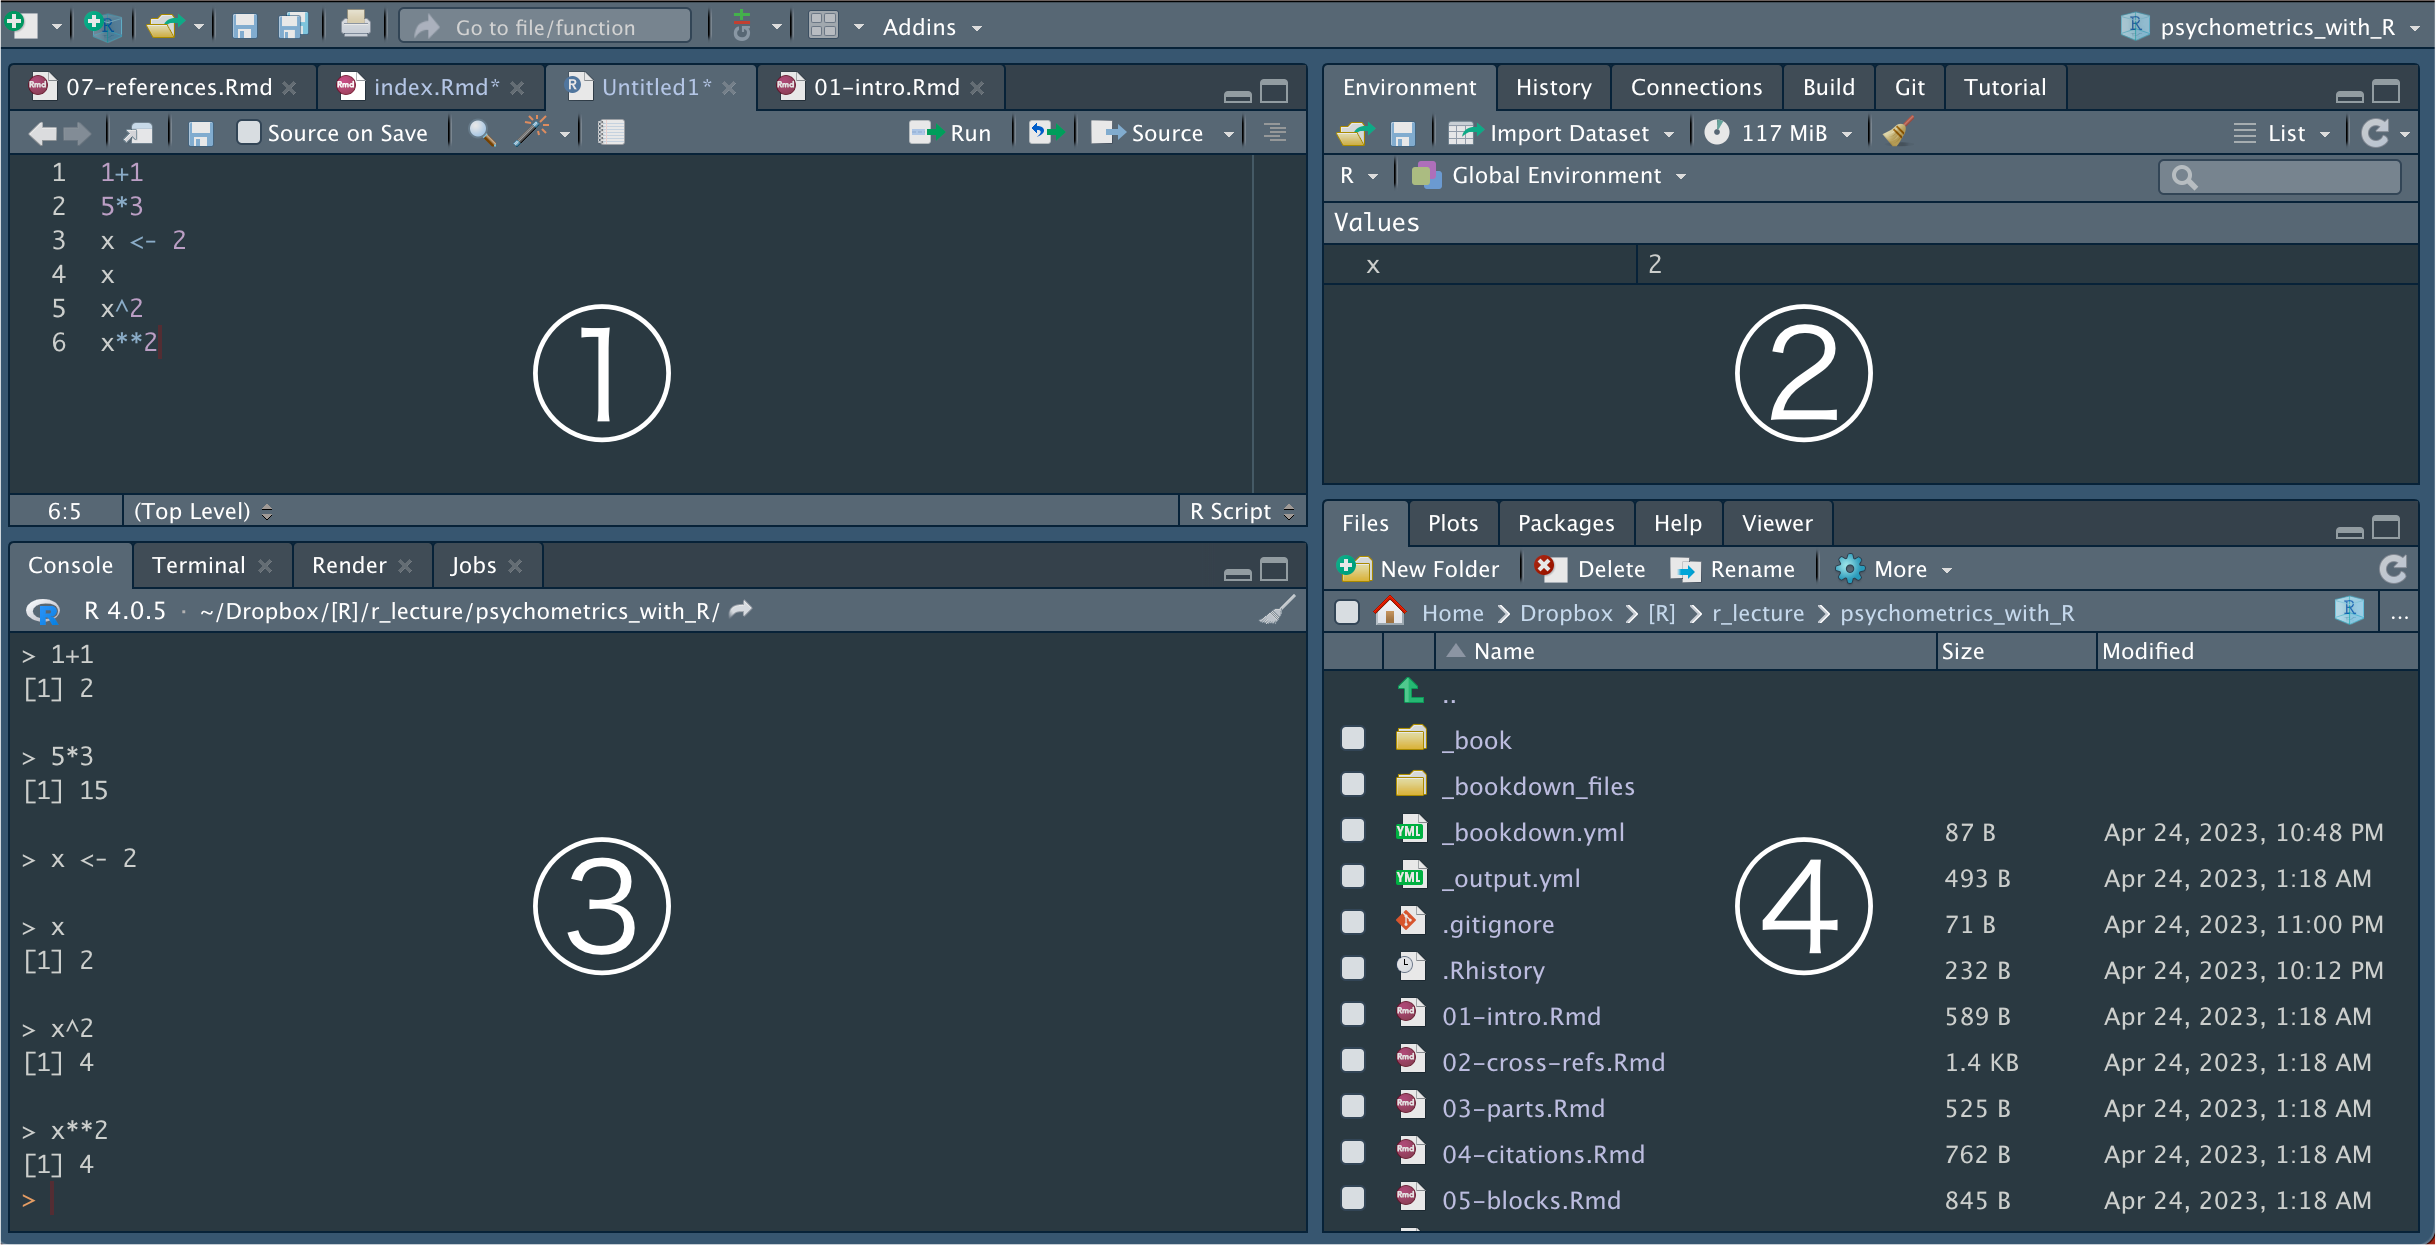
\includegraphics{./img/2_rstudio_4pane.png}

  \textbf{①左上:}メインの作業場でコードを書くところ\\
  \textbf{②右上:}変数やオブジェクトのリストが表示されたり、バージョン管理を行う\\
  \textbf{③左下:}コードの実行結果が表示されるコンソールや、各種コマンドを実行するターミナルなど\\
  \textbf{④右下:}各種ファイルやパッケージの表示、出力した図の表示など\\
  

\hypertarget{ux30b3ux30f3ux30bdux30fcux30ebux306bux76f4ux63a5ux6253ux3061ux8fbcux3080}{%
\section{コンソールに直接打ち込む}\label{ux30b3ux30f3ux30bdux30fcux30ebux306bux76f4ux63a5ux6253ux3061ux8fbcux3080}}

\begin{itemize}
\tightlist
\item
  RStudioの左下のペーンを見る\\
\item
  Consoleのタブが選択されていることを確認
\item
  簡単な足し算を実行しよう
\item
  最下段の\texttt{\textgreater{}}のあとに\texttt{1+1}と打ち込み\textbf{Enter(macはreturn)}を押す
\item
  \texttt{{[}1{]}\ 2}と返ってくる
\item
  \texttt{2}の部分が\texttt{1+1}の計算結果(\texttt{{[}1{]}}は1行目という意味)
\end{itemize}

\hypertarget{rux30b9ux30afux30eaux30d7ux30c8ux3092ux4f7fux3046}{%
\section{Rスクリプトを使う}\label{rux30b9ux30afux30eaux30d7ux30c8ux3092ux4f7fux3046}}

\begin{itemize}
\tightlist
\item
  コンソールに書いたコードは、Rstudioを終了すると消える\\
  (実際に終了して再起動してみよう)\\
\item
  だから、保存可能な\textbf{Rスクリプト}にコードを書くことが多い
\end{itemize}

\hypertarget{rux30b9ux30afux30eaux30d7ux30c8ux306bux66f8ux304f}{%
\paragraph*{Rスクリプトに書く:}\label{rux30b9ux30afux30eaux30d7ux30c8ux306bux66f8ux304f}}
\addcontentsline{toc}{paragraph}{Rスクリプトに書く:}

\begin{itemize}
\tightlist
\item
  RStudioの左上の
  をクリックし、「R Script」を選択
\item
  空のRスクリプトファイルが作成され、左上のペーンに表示される
\item
  1行目に\texttt{1+1}と入力して\textbf{ctrl+Enter(macはcommand+return)}を押す\\
  ( をクリックしても良い)
\item
  左下のペーンのコンソールに結果(\texttt{{[}1{]}\ 2})が表示される
\end{itemize}

\hypertarget{ux4fddux5b58}{%
\paragraph*{保存:}\label{ux4fddux5b58}}
\addcontentsline{toc}{paragraph}{保存:}

\begin{itemize}
\tightlist
\item
  Rスクリプトは\textbf{ctrl+s(macはcommand+s)}で好きな時に保存できる
\item
  初回はファイル名と保存場所も決める
\item
  試しに、保存したRスクリプトのタブを閉じてみよう
  (タブの右側の×をクリック)
\item
  左上の をクリックし、保存したRスクリプトのファイルを選択\\
\item
  Rスクリプトが先ほど保存した状態で開く
\end{itemize}

\hypertarget{ux3055ux3089ux306bux66f8ux304f}{%
\paragraph*{さらに書く!:}\label{ux3055ux3089ux306bux66f8ux304f}}
\addcontentsline{toc}{paragraph}{さらに書く!:}

\begin{itemize}
\tightlist
\item
  続けて、簡単な引き算を実行しよう
\item
  2行目に\texttt{5-2}と入力する
\item
  2行目にカーソルを合わせて\textbf{ctrl+Enter}を押す
\item
  2行目の計算結果(\texttt{{[}1{]}\ 3})が表示される
\item
  1行目にカーソルを合わせて\textbf{ctrl+Enter}を押す
\item
  1行目の計算結果(\texttt{{[}1{]}\ 2})が表示される
\item
  つまり、実行したい行にカーソルを合わせて\textbf{ctrl+Enter}を押せば良い
\item
  全ての行を一括で実行したいなら\textbf{ctrl+shift+Enter(macはcommand+shift+return)}
\item
  一部分だけ実行したいなら、下図のように実行したい行だけ選択して\textbf{ctrl+Enter}
\end{itemize}

\hypertarget{rux30b9ux30afux30eaux30d7ux30c8ux3092ux4f7fux3046ux30e1ux30eaux30c3ux30c8}{%
\paragraph*{Rスクリプトを使うメリット:}\label{rux30b9ux30afux30eaux30d7ux30c8ux3092ux4f7fux3046ux30e1ux30eaux30c3ux30c8}}
\addcontentsline{toc}{paragraph}{Rスクリプトを使うメリット:}

\begin{enumerate}
\def\labelenumi{\arabic{enumi}.}
\tightlist
\item
  コードが保存できる(毎回書き直さなくて良い!)
\item
  長く複雑なコードを書いたり、管理するのが楽\\
\item
  他の人に配布できる(分析を再現してもらいやすい)\\
  などなど\ldots{}
\end{enumerate}

\hypertarget{ux30d7ux30edux30b8ux30a7ux30afux30c8ux7ba1ux7406}{%
\section{プロジェクト管理}\label{ux30d7ux30edux30b8ux30a7ux30afux30c8ux7ba1ux7406}}

\begin{itemize}
\tightlist
\item
  研究プロジェクトが進むと、ひとつのRスクリプトだけでは管理しきれなくなる
\item
  \textbf{プロジェクト}を使えば、複数のRスクリプトや関連データなどを一つのフォルダにまとめて効率よく管理できる
\end{itemize}

\hypertarget{ux30d7ux30edux30b8ux30a7ux30afux30c8ux306eux4f5cux6210}{%
\paragraph*{プロジェクトの作成:}\label{ux30d7ux30edux30b8ux30a7ux30afux30c8ux306eux4f5cux6210}}
\addcontentsline{toc}{paragraph}{プロジェクトの作成:}

\begin{itemize}
\tightlist
\item
  左上の をクリックし、「New Directry」→「New Project」の順に選択\\
\item
  次の画面で①プロジェクト名と、その②作成場所を指定して③「Create Project」
\end{itemize}

\begin{itemize}
\tightlist
\item
  指定した場所に、指定したプロジェクト名のフォルダができているのを確認しよう
\item
  そのフォルダの中に「プロジェクト名.Rproj」というファイルができているのを確認しよう
\item
  以下は、macでDocumentフォルダ内にsugoi\_projectというプロジェクトを作った例
\end{itemize}

\begin{itemize}
\tightlist
\item
  初めはご利益がわかりにくいが、研究プロジェクトごとにプロジェクトを作るクセをつけよう
\item
  そして、次の心得に従い、プロジェクト上で作業をするようにしよう!
\end{itemize}

\begin{enumerate}
\def\labelenumi{\arabic{enumi}.}
\tightlist
\item
  毎回「プロジェクト名.Rproj」をダブルクリックしてRstudioを起動
\item
  関連するファイルはプロジェクト名のフォルダにまとめて一元管理
\end{enumerate}

\hypertarget{ux57faux672cux64cdux4f5c}{%
\chapter{基本操作}\label{ux57faux672cux64cdux4f5c}}

\begin{itemize}
\tightlist
\item
  現状では、ベースにした森先生の資料の丸写しです
\item
  GW明けまでに完成させるので、外に出さないでください
\item
  森先生の以下の動画を参考にしてください
\item
  GW明けまでに全ての練習問題のコードをひとつのRスクリプトに書いて提出
\end{itemize}

\hypertarget{ux30aaux30d6ux30b8ux30a7ux30afux30c8}{%
\section{オブジェクト}\label{ux30aaux30d6ux30b8ux30a7ux30afux30c8}}

Rで使用するあらゆる「モノ」はオブジェクト(object)と呼ばれ管理されます。 オブジェクトの準備からRの分析はスタートします。まずは、オブジェクトを準備してみましょう。

\begin{Shaded}
\begin{Highlighting}[]
\NormalTok{first\_object }\OtherTok{\textless{}{-}} \DecValTok{1}
\end{Highlighting}
\end{Shaded}

オブジェクトは「名前」と「中身」で構成されます。 このコマンドでは、first\_objectという名前のオブジェクトに「1」という数値を入れています。 \textless-(不等号・ハイフン)は矢印を表していて、左側の名前のオブジェクトに右側の「モノ」を代入する命令です。 このコマンドを実行しても何も表示されませんが、それでOKです。

オブジェクトの名前を指定すると、オブジェクトの中身を表示させることができます。

\begin{Shaded}
\begin{Highlighting}[]
\NormalTok{first\_object}
\end{Highlighting}
\end{Shaded}

\begin{verbatim}
## [1] 1
\end{verbatim}

{[}1{]}は「1行目」を意味しています。そのあとの「1」が中身です。

また、代入する命令を()でくくることで、代入させつつ表示させることができます。 second\_objectに2を入れて表示させてみましょう。

\begin{Shaded}
\begin{Highlighting}[]
\NormalTok{(second\_object }\OtherTok{\textless{}{-}} \DecValTok{2}\NormalTok{)}
\end{Highlighting}
\end{Shaded}

\begin{verbatim}
## [1] 2
\end{verbatim}

文字列をオブジェクトに入れることもできます。 この場合、文字列を''\,``(引用符)でくくります。

\begin{Shaded}
\begin{Highlighting}[]
\NormalTok{first\_string\_object }\OtherTok{\textless{}{-}} \StringTok{"Ritsumeikan University"}
\NormalTok{first\_string\_object}
\end{Highlighting}
\end{Shaded}

\begin{verbatim}
## [1] "Ritsumeikan University"
\end{verbatim}

ここでは、first\_string\_objectという名前のオブジェクトに、文字列''Ritsumeikan University''を入れています。

オブジェクトに入れるものは1つの値ではなく、複数の値にすることもできます。 複数の値を並べたものは「ベクトル」と呼ばれます。 ベクトルはc()でまとめます。

\begin{Shaded}
\begin{Highlighting}[]
\NormalTok{first\_vector\_object }\OtherTok{\textless{}{-}} \FunctionTok{c}\NormalTok{(}\DecValTok{1}\NormalTok{, }\DecValTok{2}\NormalTok{, }\DecValTok{3}\NormalTok{, }\DecValTok{4}\NormalTok{, }\DecValTok{5}\NormalTok{)}
\NormalTok{first\_vector\_object}
\end{Highlighting}
\end{Shaded}

\begin{verbatim}
## [1] 1 2 3 4 5
\end{verbatim}

ここでは、first\_vector\_objectというオブジェクトに、1から5までの数値を代入しています。 文字列のベクトルも作ることができるので、試してみてください。

\textbf{練習問題}

\begin{itemize}
\tightlist
\item
  third\_objectという名前のオブジェクトに10000を代入し、確認してください。\\
\item
  my\_nameという名前のオブジェクトにあなたの名前(文字列)を代入し、確認してください。\\
\item
  second\_vector\_objectという名前のオブジェクトに数値のベクトル1, 1, 2, 3, 5, 8を代入し、確認してください。
\end{itemize}

\hypertarget{ux7c21ux5358ux306aux8a08ux7b97}{%
\section{簡単な計算}\label{ux7c21ux5358ux306aux8a08ux7b97}}

Rでの簡単な計算をしてみましょう。足し算・引き算は日常用語と同じく+, -を用います。

\begin{Shaded}
\begin{Highlighting}[]
\DecValTok{1} \SpecialCharTok{+} \DecValTok{1}
\end{Highlighting}
\end{Shaded}

\begin{verbatim}
## [1] 2
\end{verbatim}

\begin{Shaded}
\begin{Highlighting}[]
\DecValTok{5} \SpecialCharTok{{-}} \DecValTok{2}
\end{Highlighting}
\end{Shaded}

\begin{verbatim}
## [1] 3
\end{verbatim}

掛け算は*、割り算は/を使います。また、累乗は\^{}です。日常用語とは異なりますが、Excelと同じです。

\begin{Shaded}
\begin{Highlighting}[]
\DecValTok{2} \SpecialCharTok{*} \DecValTok{3}
\end{Highlighting}
\end{Shaded}

\begin{verbatim}
## [1] 6
\end{verbatim}

\begin{Shaded}
\begin{Highlighting}[]
\DecValTok{10} \SpecialCharTok{/} \DecValTok{2}
\end{Highlighting}
\end{Shaded}

\begin{verbatim}
## [1] 5
\end{verbatim}

\begin{Shaded}
\begin{Highlighting}[]
\DecValTok{4} \SpecialCharTok{\^{}} \DecValTok{2}
\end{Highlighting}
\end{Shaded}

\begin{verbatim}
## [1] 16
\end{verbatim}

ここまでは数値同士で計算させていましたが、数値を代入したオブジェクトも使うことができます。例えば、`age'に年齢を代入しておき、10年後の年齢を計算させてみましょう。

\begin{Shaded}
\begin{Highlighting}[]
\NormalTok{age }\OtherTok{\textless{}{-}} \DecValTok{20}
\NormalTok{age }\SpecialCharTok{+} \DecValTok{10}
\end{Highlighting}
\end{Shaded}

\begin{verbatim}
## [1] 30
\end{verbatim}

ここまでは計算結果を単に表示させていました。計算結果をオブジェクトに代入することもできます。 例えば、1 + 1の結果をone\_plus\_oneというオブジェクトに代入してみましょう。

\begin{Shaded}
\begin{Highlighting}[]
\NormalTok{one\_plus\_one }\OtherTok{\textless{}{-}} \DecValTok{1} \SpecialCharTok{+} \DecValTok{1}
\NormalTok{one\_plus\_one}
\end{Highlighting}
\end{Shaded}

\begin{verbatim}
## [1] 2
\end{verbatim}

オブジェクトone\_plus\_oneには計算結果2が代入されています。

\textbf{練習問題}

\begin{itemize}
\tightlist
\item
  オブジェクトaに3を、オブジェクトbに4を代入してください。
\item
  a, bそれぞれを2乗したものの和をとり、結果が25となることを確認してください。
\end{itemize}

\hypertarget{ux95a2ux6570}{%
\section{5.3 関数}\label{ux95a2ux6570}}

Rではオブジェクトから別のオブジェクトを生成するために「関数(function)」を用います。 関数の使い方に慣れていきましょう。 関数は関数名(引数)という構造で使います。 引数(argument)は「ひきすう」と読みます。

ここでは、簡単な関数の例を紹介します。 その他の関数はその都度紹介します。

\hypertarget{ux6570ux5024ux306bux5bfeux3059ux308bux95a2ux6570}{%
\subsection{数値に対する関数}\label{ux6570ux5024ux306bux5bfeux3059ux308bux95a2ux6570}}

皆さんが数学で勉強してきた関数をRの関数として使うことができます。例えば平方根をとる関数sqrt()を使ってみましょう。

\begin{Shaded}
\begin{Highlighting}[]
\FunctionTok{sqrt}\NormalTok{(}\DecValTok{4}\NormalTok{)}
\end{Highlighting}
\end{Shaded}

\begin{verbatim}
## [1] 2
\end{verbatim}

ここでは、sqrt()が関数、引数は4です。4の平方根をとった結果として2が表示されています。他の数式として例えば自然対数をとるlog()があります。

\textbf{練習問題}

\begin{itemize}
\tightlist
\item
  オブジェクトaに3を、オブジェクトbに4を代入してください。(前の問題と同様)\\
\item
  a, bそれぞれの2乗して和をとったものの平方根をとり、結果が5となることを確認してください。\\
  ヒント:前の問題の計算全体をsqrt()のかっこでくくってください。
\end{itemize}

\hypertarget{ux30d9ux30afux30c8ux30ebux306bux5bfeux3059ux308bux95a2ux6570}{%
\subsection{ベクトルに対する関数}\label{ux30d9ux30afux30c8ux30ebux306bux5bfeux3059ux308bux95a2ux6570}}

関数の引数は数値だけでなく、ベクトルをとることもできます。統計分析ではこちらをよく使います。例えば、年齢のデータが入ったベクトル\texttt{age\_vector\ \textless{}-\ c(18,\ 21,\ 22,\ 23,\ 34)}を考えます。

例えば、ベクトルの最小値を取り出す\texttt{min()}を使ってみましょう。

\begin{Shaded}
\begin{Highlighting}[]
\NormalTok{age\_vector }\OtherTok{\textless{}{-}} \FunctionTok{c}\NormalTok{(}\DecValTok{18}\NormalTok{, }\DecValTok{21}\NormalTok{, }\DecValTok{22}\NormalTok{, }\DecValTok{23}\NormalTok{, }\DecValTok{34}\NormalTok{)}
\FunctionTok{min}\NormalTok{(age\_vector)}
\end{Highlighting}
\end{Shaded}

\begin{verbatim}
## [1] 18
\end{verbatim}

一番年齢が若い人が18歳であることが確認できます。最大値を取り出すのは\texttt{max()}です。

心理学統計法で学んだ平均・標準偏差などの統計量も計算することができます。平均は\texttt{mean()}、中央値は\texttt{median()}、(不偏)標準偏差は\texttt{sd()}を使います。

\begin{Shaded}
\begin{Highlighting}[]
\FunctionTok{mean}\NormalTok{(age\_vector)}
\end{Highlighting}
\end{Shaded}

\begin{verbatim}
## [1] 23.6
\end{verbatim}

\begin{Shaded}
\begin{Highlighting}[]
\FunctionTok{median}\NormalTok{(age\_vector)}
\end{Highlighting}
\end{Shaded}

\begin{verbatim}
## [1] 22
\end{verbatim}

\begin{Shaded}
\begin{Highlighting}[]
\FunctionTok{sd}\NormalTok{(age\_vector)}
\end{Highlighting}
\end{Shaded}

\begin{verbatim}
## [1] 6.107373
\end{verbatim}

\textbf{練習問題}

\begin{itemize}
\tightlist
\item
  オブジェクトincome\_vectorに数値のベクトル10, 100, 1000, 10000, 100000を代入してください。\\
\item
  income\_vectorの平均・中央値・標準偏差をそれぞれ求めてください。
\end{itemize}

\hypertarget{ux30c7ux30fcux30bfux30d5ux30ecux30fcux30e0}{%
\section{データフレーム}\label{ux30c7ux30fcux30bfux30d5ux30ecux30fcux30e0}}

多くのデータは、表形式でまとめられます。 縦方向に観測値を、横方向に変数を並べたデータのことをRではデータフレームと呼びます。

例として、年齢のベクトルage\_vectorと性別のベクトルgender\_vectorを合わせてデータフレームを作成してみましょう。 データフレームを作成する関数は\texttt{data.frame()}です。

\begin{Shaded}
\begin{Highlighting}[]
\NormalTok{age }\OtherTok{\textless{}{-}} \FunctionTok{c}\NormalTok{(}\DecValTok{18}\NormalTok{, }\DecValTok{21}\NormalTok{, }\DecValTok{22}\NormalTok{, }\DecValTok{23}\NormalTok{, }\DecValTok{34}\NormalTok{) }\CommentTok{\#年齢のベクトルの作成}
\NormalTok{gender }\OtherTok{\textless{}{-}} \FunctionTok{c}\NormalTok{(}\StringTok{"female"}\NormalTok{, }\StringTok{"male"}\NormalTok{, }\StringTok{"male"}\NormalTok{, }\StringTok{"female"}\NormalTok{, }\StringTok{"female"}\NormalTok{) }\CommentTok{\#性別のベクトルの作成}
\NormalTok{first\_dataframe }\OtherTok{\textless{}{-}} \FunctionTok{data.frame}\NormalTok{(age, gender)}
\NormalTok{first\_dataframe}
\end{Highlighting}
\end{Shaded}

\begin{verbatim}
##   age gender
## 1  18 female
## 2  21   male
## 3  22   male
## 4  23 female
## 5  34 female
\end{verbatim}

1人目が18歳の女性、2人目が21歳の男性\ldots を表すデータフレームが作成できました。 後ほどExcelファイルなどからデータのRにインポートする方法を学びますが、その際は自動的にデータフレームとしてインポートされます。

データ分析の際に、データフレームのうち特定の変数だけを使いたい場合がよくあります。 その際は、データフレーム名\$変数名と表記することで、特定の変数を使うことができます。 例えば、先ほど作成したfirst\_dataframeから性別の変数のみを見てみましょう。

\begin{Shaded}
\begin{Highlighting}[]
\NormalTok{first\_dataframe}\SpecialCharTok{$}\NormalTok{gender}
\end{Highlighting}
\end{Shaded}

\begin{verbatim}
## [1] "female" "male"   "male"   "female" "female"
\end{verbatim}

性別のベクトルを取り出すことができました。 関数と組み合わせると、年齢の平均値を以下のように計算できます。

\begin{Shaded}
\begin{Highlighting}[]
\FunctionTok{mean}\NormalTok{(first\_dataframe}\SpecialCharTok{$}\NormalTok{age)}
\end{Highlighting}
\end{Shaded}

\begin{verbatim}
## [1] 23.6
\end{verbatim}

\textbf{練習問題}

\begin{itemize}
\tightlist
\item
  オブジェクトincomeに数値のベクトル10, 100, 1000, 10000, 100000を代入してください。\\
\item
  オブジェクトcityに文字列のベクトル''ibaraki'', ``takatsuki'', ``ibaraki'', ``takatsuki'', ``takatsuki''を代入してください。\\
\item
  incomeとcityを合わせたデータフレームincome\_dataを作成してください。\\
\item
  income\_dataを用いて、incomeの中央値を求めてください。
\end{itemize}

\hypertarget{ux30c7ux30fcux30bfux306eux8aadux307fux8fbcux307f}{%
\chapter{データの読み込み}\label{ux30c7ux30fcux30bfux306eux8aadux307fux8fbcux307f}}

\begin{itemize}
\tightlist
\item
  現状では、ベースにした森先生の資料の丸写しです
\item
  GW明けまでに完成させるので、外に出さないでください
\item
  森先生の以下の動画を参考にしてください
\item
  GW明けまでに全ての練習問題のコードをひとつのRスクリプトに書いて提出
\end{itemize}

データ分析のためには、データをRStudioにインポート(読み込み)させなければなりません。インポートの方法は、持っているデータのファイル形式によって変わります。

\hypertarget{ux30a4ux30f3ux30ddux30fcux30c8ux306eux6e96ux5099}{%
\section{インポートの準備}\label{ux30a4ux30f3ux30ddux30fcux30c8ux306eux6e96ux5099}}

インポートしたいファイルは、プロジェクトと同じフォルダに入れておきましょう。 プロジェクトはChapter 2で学習しています。

インポートしたいファイルの形式も確認しておきましょう。 代表的な形式として、CSVファイル(.csv)、Excelファイル(.xlsx, .xls)があります。 拡張子が表示されていない場合はこちらを参考に表示させるようにしましょう。

インポートの前に、ファイルの1行目は変数名(英語)にしておきましょう。

\hypertarget{ux30d5ux30a1ux30a4ux30ebux5f62ux5f0fux5225ux306eux30a4ux30f3ux30ddux30fcux30c8ux65b9ux6cd5}{%
\section{ファイル形式別のインポート方法}\label{ux30d5ux30a1ux30a4ux30ebux5f62ux5f0fux5225ux306eux30a4ux30f3ux30ddux30fcux30c8ux65b9ux6cd5}}

\hypertarget{csvux30d5ux30a1ux30a4ux30ebux306eux5834ux5408.csv}{%
\subsection{CSVファイルの場合(.csv)}\label{csvux30d5ux30a1ux30a4ux30ebux306eux5834ux5408.csv}}

CSVファイルの場合は、\texttt{read.csv}を用います。ファイルの名前がsotsuron.csvの場合、以下のように実行します。

\begin{Shaded}
\begin{Highlighting}[]
\NormalTok{data\_original }\OtherTok{\textless{}{-}} \FunctionTok{read.csv}\NormalTok{(}\StringTok{"sotsuron.csv"}\NormalTok{)}
\end{Highlighting}
\end{Shaded}

これは、csvファイルの内容をdata\_originalというオブジェクトに格納しています。 オブジェクト名は自由につけることができますが、わかりやすいものにしましょう。 ここでは、インポートした元データであることを明示するため、data\_originalという名前にしています。

\textbf{練習問題}

\begin{itemize}
\tightlist
\item
  以下から「tidy\_data.csv」をダウンロード
  \url{https://www.dropbox.com/s/wm46esg4dicye8j/tidy_data.csv?dl=0}\\
\item
  \texttt{read.csv}を使って読み込み、dataというオブジェクトに格納
\end{itemize}

\hypertarget{ux30a4ux30f3ux30ddux30fcux30c8ux3057ux305fux30c7ux30fcux30bfux306eux78baux8a8d}{%
\section{インポートしたデータの確認}\label{ux30a4ux30f3ux30ddux30fcux30c8ux3057ux305fux30c7ux30fcux30bfux306eux78baux8a8d}}

上の練習問題のデータがきちんとインポートされたかどうか、確認しておきましょう。

右上のペーンの``Environment''に新しいオブジェクトができているか確認(上の例ではdata)
クリックして左上のペーンに出てくるか確認
\texttt{head(data)}で先頭のデータを確認
\texttt{str(data)}で各変数の「型」(後で説明)を確認

  \bibliography{book.bib,packages.bib}

\end{document}
